\documentclass{beamer}

\usepackage[utf8]{inputenc}
\usepackage{graphicx}
\usepackage{multimedia}
\usepackage{url}

\usetheme{Copenhagen}
\useoutertheme{sidebar}

\title{Jeu du Pérudo}
\author{H4104 - Dragibus}
\institute{INSA de Lyon}
\logo{
\includegraphics[height=8mm, width=14mm]{logo}}

\begin{document}

\begin{frame}
  \titlepage
\end{frame}

\begin{frame}
  \frametitle{Sommaire}
  \tableofcontents[hideallsubsections]
\end{frame}

\section{Mécanisme du jeu}

\begin{frame}
  \frametitle{Principe}

  \begin{figure}
    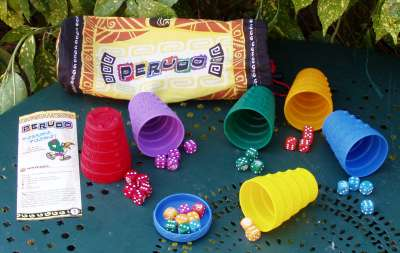
\includegraphics[scale=0.4]{perudo}
  \end{figure}

  \begin{itemize}
    \item jeu de dés
    \item multijoueur, entre 2 et 6 (ou plus) joueurs
    \item deviner le nombre de dés d'une valeur, connaissant seulement ses
      propres dés
    \item dernier joueur ayant des dés gagne la partie
  \end{itemize}
\end{frame}

\begin{frame}
  \frametitle{Règles}
  $\to$ parier sur le nombre de dés en jeu \\
  \emph{(pour une certaine valeur de dé)}

  \begin{itemize}
    \item dudo : "douter", soit réfuter la mise actuelle
    \item calza : "calé", affirmer que la mise actuelle est exacte
    \item enchère : augmenter le nombre de dés ou changer la valeur du dé
  \end{itemize}

  \textbf{Exemple}
  \\
  Joueur précédent : \textit{"Je pense qu'il y a douze 5"}
  \\
  Moi :\textit{"Je pense qu'il y a treize 5"}
  \\[5mm]
  $\to$ la mise ne peut qu'\textbf{augmenter} au cours de la partie
\end{frame}

\section{Concept d'IA}

\begin{frame}
  \frametitle{Constat}

  À son tour, le joueur doit \textbf{évaluer} les différents coups possibles.
  \\[1.5cm]
  \begin{center}
    \textit{Une IA devrait fonctionner de la même manière.}
  \end{center}
\end{frame}

\begin{frame}
  \frametitle{Évaluation}

  \begin{itemize}
    \item état de soi-même (dés)
    \item état du jeu (mise précédente, historique des mises, nombre de dés)
    \item coups possibles
  \end{itemize}

  \center{$ia(EtatJoueur, EtatJeu, CoupsPossibles) \to Evaluation$}
  \\[1cm]
  \large L'IA est une \textbf{fonction d'évaluation} de l'état du jeu.
\end{frame}

\begin{frame}
  \frametitle{Combinaison}

  \begin{large}
    Permet de créer des IA complèxes à partir d'autres relativement simples.
    \\[1cm]
    Combinaison linéaire avec des coefficients de \emph{poids}, correspondant à
    la prise en compte dans la décision finale.
    $$
    IA = \left( p_i \cdot ia_i \right)_{1<i<n}
    $$
  \end{large}
\end{frame}

\section{Présentation des IA}

\begin{frame}
  \frametitle{Basiques}

  \textbf{Stochastique}
  \\
  Fonctionnement : associe à chaque coup une estimation aléatoire.
  \\
  Résultat attendu : inattendu.
  \\[1cm]
  \textbf{Minimale}
  \\
  Fonctionnement : joue à son tour le coup le moins risqué.
  \\
  Résultat attendu : taux de victoire stable et moyen.
\end{frame}

\begin{frame}
  \frametitle{Probabiliste}

  Fonctionnement : associe à chaque coup la probabilité qu'il soit présent.

  Pour un nombre de dés $n$ "inconnus", la probabilité $P(q)$ qu'il y ait
  \emph{au moins} la quantité $q$ de la valeur souhaitée est de :

  $$
  \sum\limits_{x=q}^n C(n, x) \cdot (1/6)^x \cdot (5/6)^{n-x}
  $$

  Où C(n, q) est le coefficient binomial (q parmi n).
  \\[1cm]

  Résultat attendu : taux de victoire stable et élevé.
\end{frame}

\begin{frame}
  \frametitle{Apprentissage}

  Fonctionnement : associe à chaque joueur un indice de confiance $\to$
  \textit{distance entre les mises du joueur et son jeu réel}
  \\[1cm]
  Si un joueur a une confiance de $C$ et a misé $Nb$ dés, il y a en réalité $C
  \cdot Nb$ dés.
  \\[1cm]
  Résultat attendu : croissance du taux de victoire au cours du temps.
\end{frame}

\section{Démonstration}
\begin{frame}
  \frametitle{}

  \begin{center}
    Démonstration
  \end{center}
\end{frame}

\section{Résultats et observations}

\begin{frame}
  \frametitle{IA Stochastique contre les autres}

  \begin{figure}
    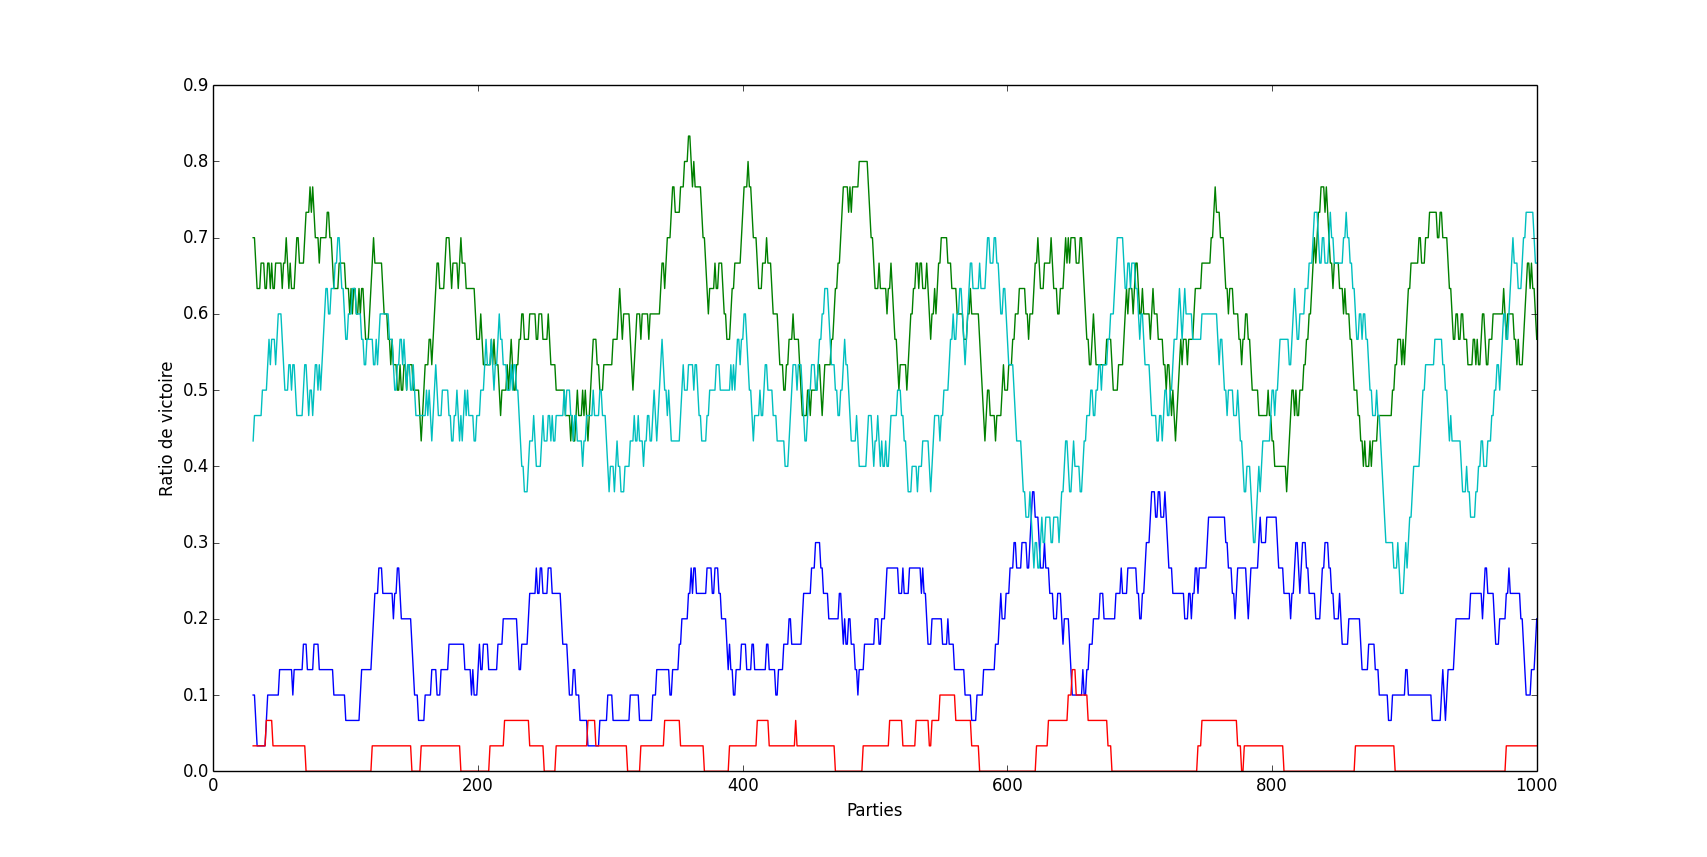
\includegraphics[scale=0.265]{plot/ivre}
  \end{figure}
\end{frame}

\begin{frame}
  \frametitle{IA Minimale contre les autres}
  \begin{figure}
    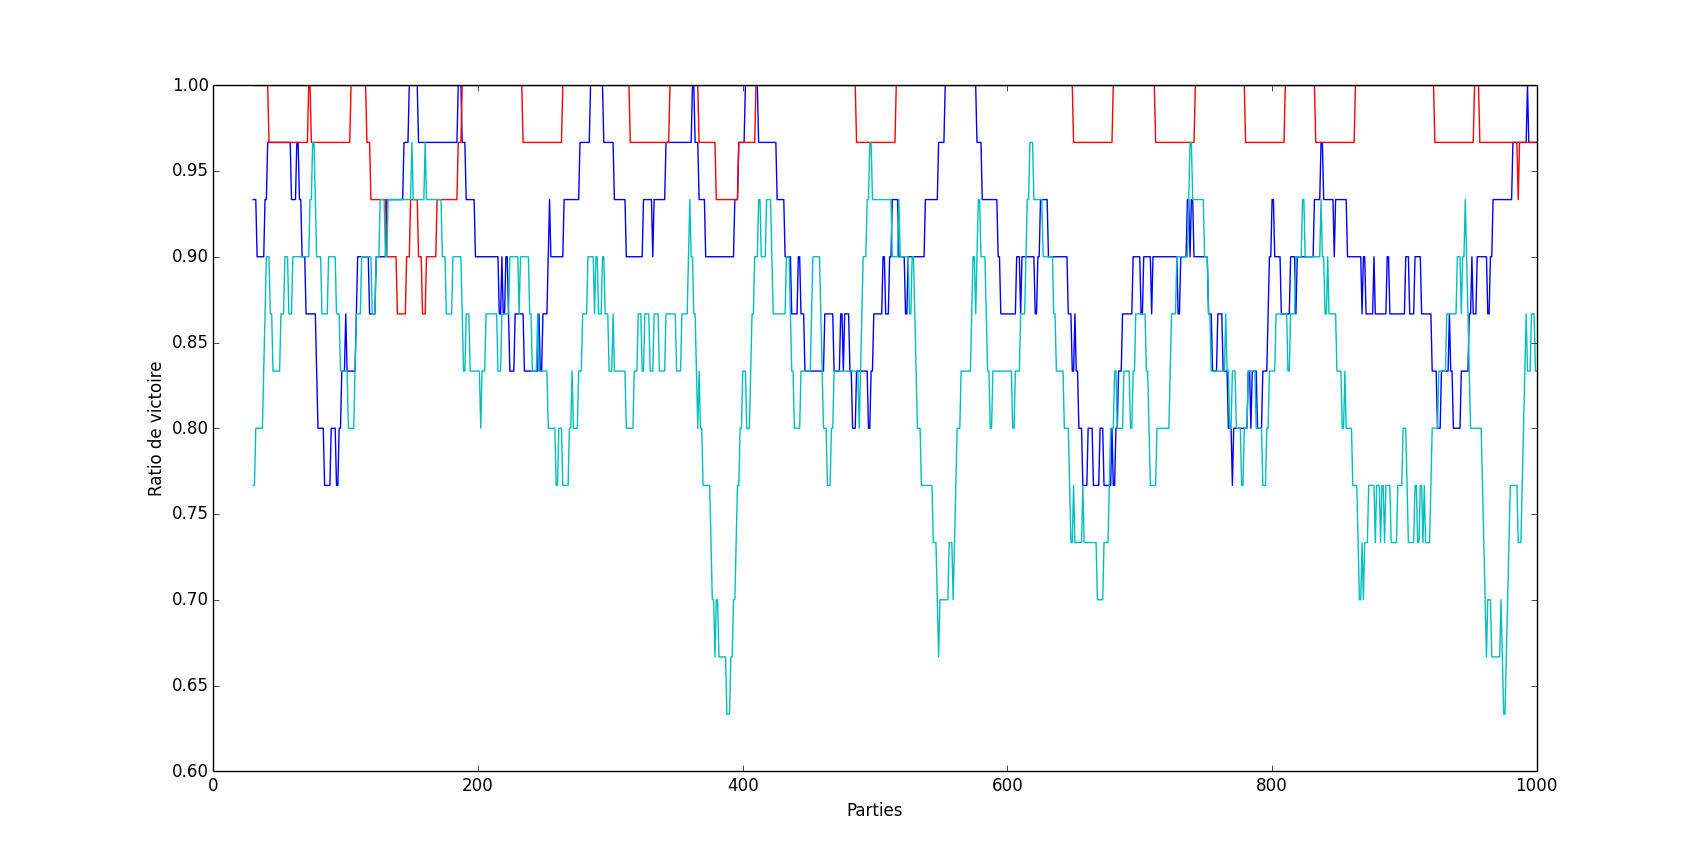
\includegraphics[scale=0.265]{plot/debile}
    \caption{
      \label{fig_debile} Le taux de gain est élevé et au dessus de notre attente.
    }
  \end{figure}
\end{frame}

\begin{frame}
  \frametitle{IA Probabiliste contre les autres}
  \begin{figure}
    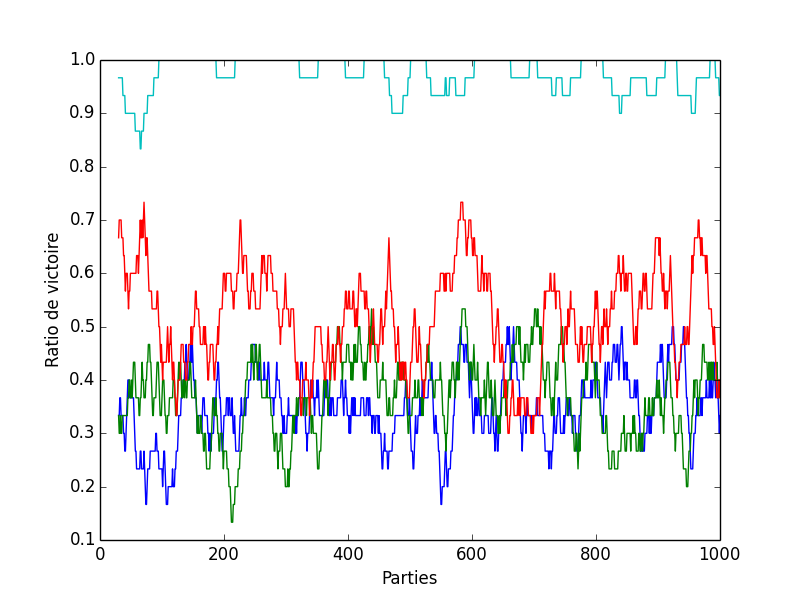
\includegraphics[scale=0.265]{plot/stats}
    \caption{
      \label{fig_stats} On confirme la stabilité de l'intelligence.
    }
  \end{figure}
\end{frame}

\begin{frame}
  \frametitle{IA Apprentissage contre les autres}
  \begin{figure}
    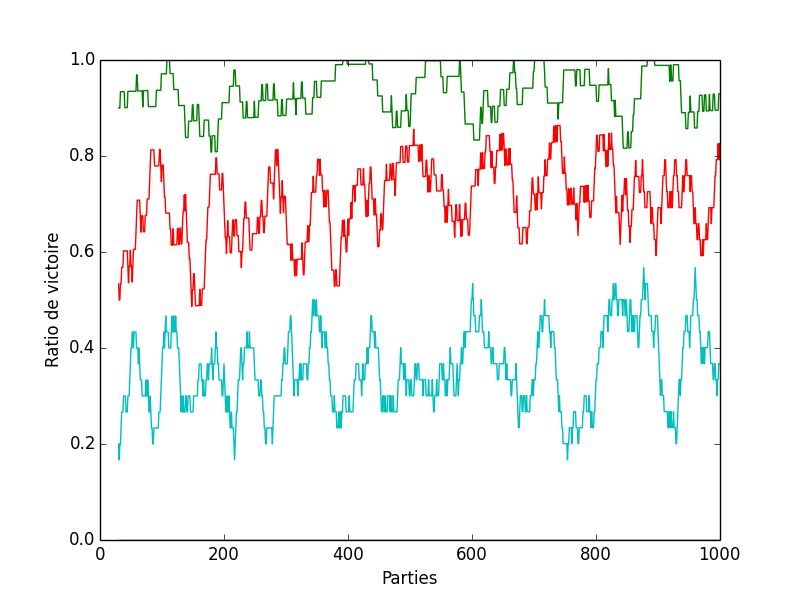
\includegraphics[scale=0.265]{plot/eleve}
    \caption{
      \label{fig_eleve} On observe une légère croissance du taux de victoires.
    }
  \end{figure}
\end{frame}

\begin{frame}
  \frametitle{Classement des meilleures IA}
  \begin{center}
    \begin{tabular}{|r|l|l|l|l|l|}
      \hline
      \#  &  Mini.     &  Appr.  &  Stats  &  Stoch.  &  Score  \\
      \hline
      1   &  0.5       &  0.0    &  0.5    &  0       &  83762  \\
      2   &  5.82e-05  &  0.49   &  0.5    &  0       &  82793  \\
      3   &  2.98e-07  &  0.49   &  0.5    &  0       &  82774  \\
      4   &  0.01      &  0.49   &  0.5    &  0       &  82656  \\
      5   &  0.0       &  0.5    &  0.5    &  0       &  82618  \\
      6   &  1.14e-09  &  0.49   &  0.5    &  0       &  82251  \\
      7   &  0.5       &  0.0    &  0.5    &  0.5     &  74322  \\
      8   &  1.19e-07  &  0.19   &  0.8    &  0       &  57273  \\
      9   &  4.59e-10  &  0.19   &  0.8    &  0       &  57246  \\
      10  &  2.33e-05  &  0.19   &  0.8    &  0       &  57117  \\
      \hline
    \end{tabular}
  \end{center}
\end{frame}

\begin{frame}
  \frametitle{La meilleure IA contre toutes les autres}

  \center Combinaison 0.5/0/0.5/0

  \begin{figure}
    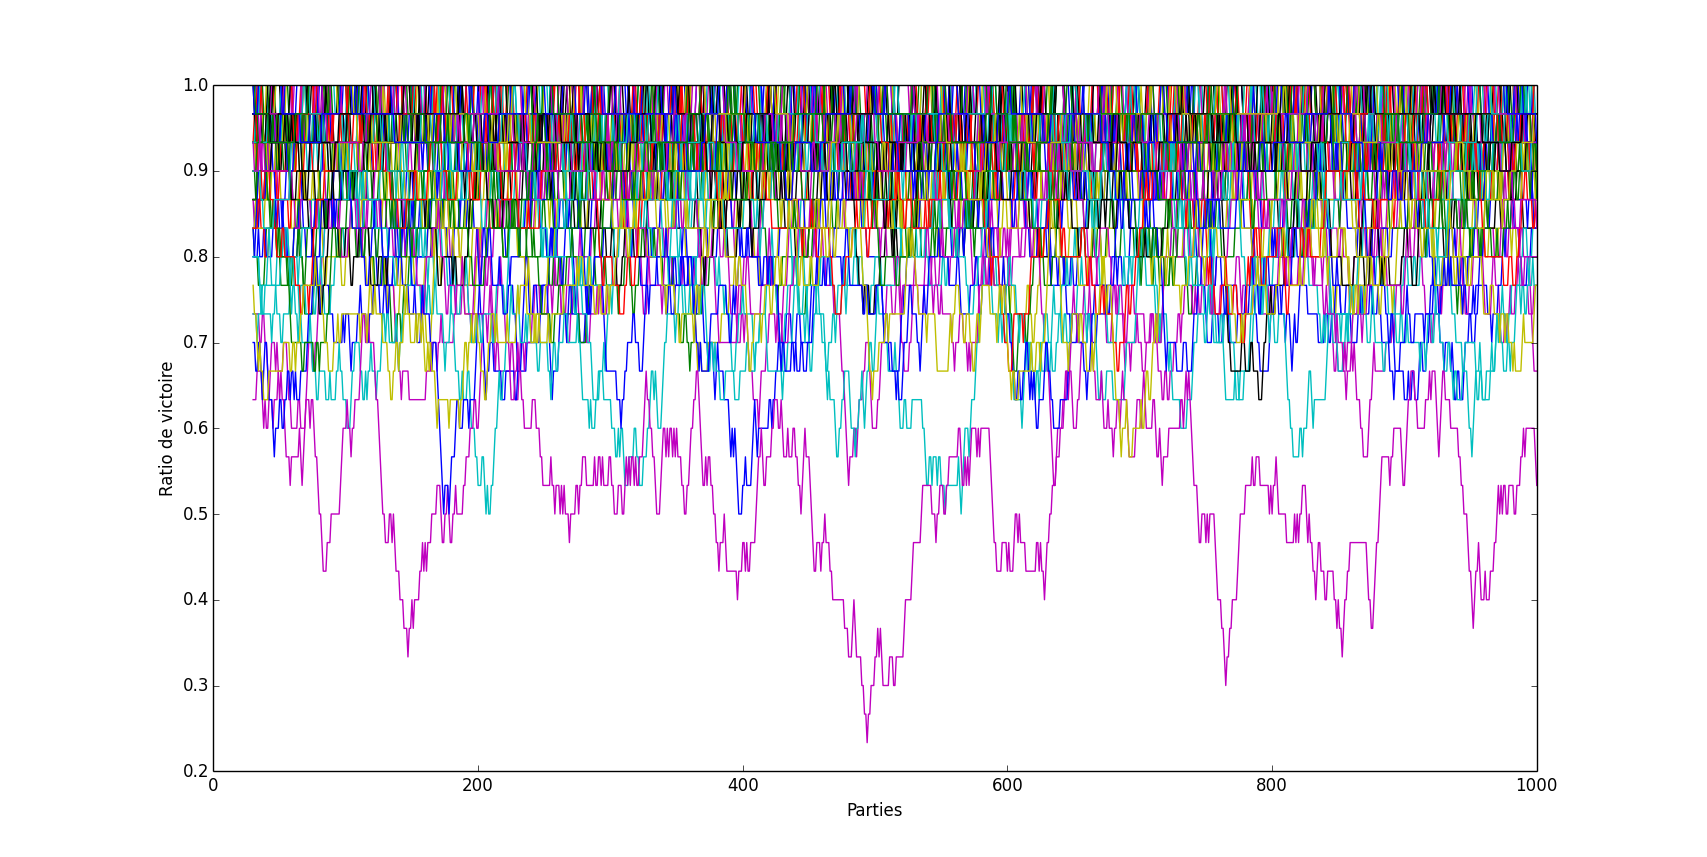
\includegraphics[scale=0.265, trim=0 2cm 0 0]{plot/best}
  \end{figure}
\end{frame}

\begin{frame}
  \frametitle{Observation de l'apprentissage}

  \center Combinaison 0/1/0/0.5

  \begin{figure}
    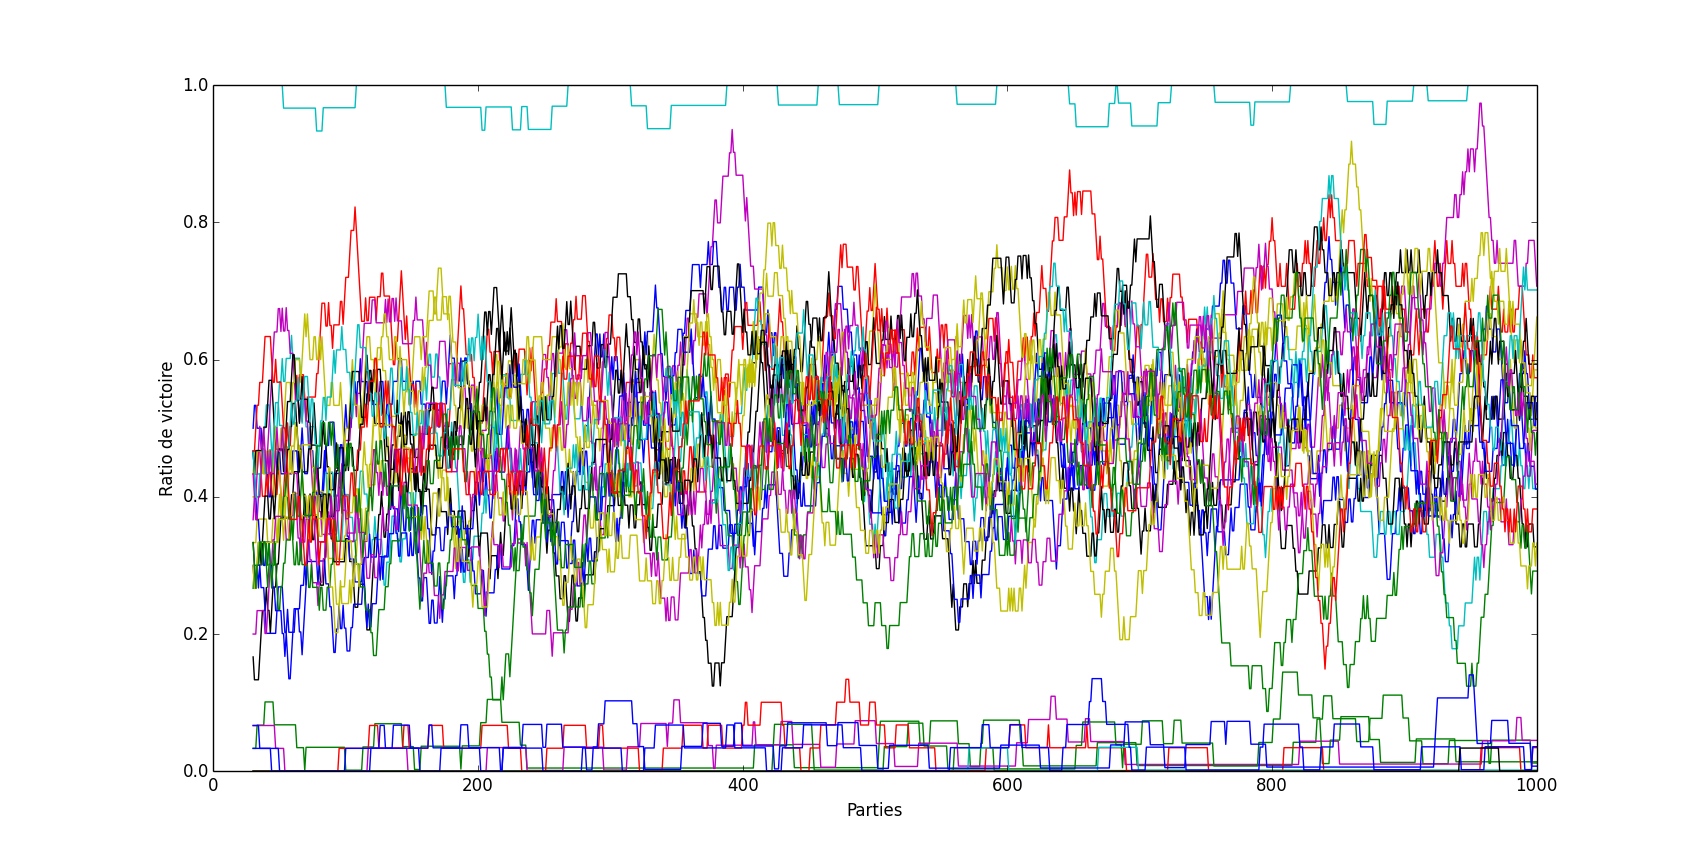
\includegraphics[scale=0.265, trim=0 2cm 0 0]{plot/eleve2}
  \end{figure}
\end{frame}

\begin{frame}
  \frametitle{Cas particulier intéressant}

  \center Combinaison 0/0.5/0.5/0

  \begin{figure}
    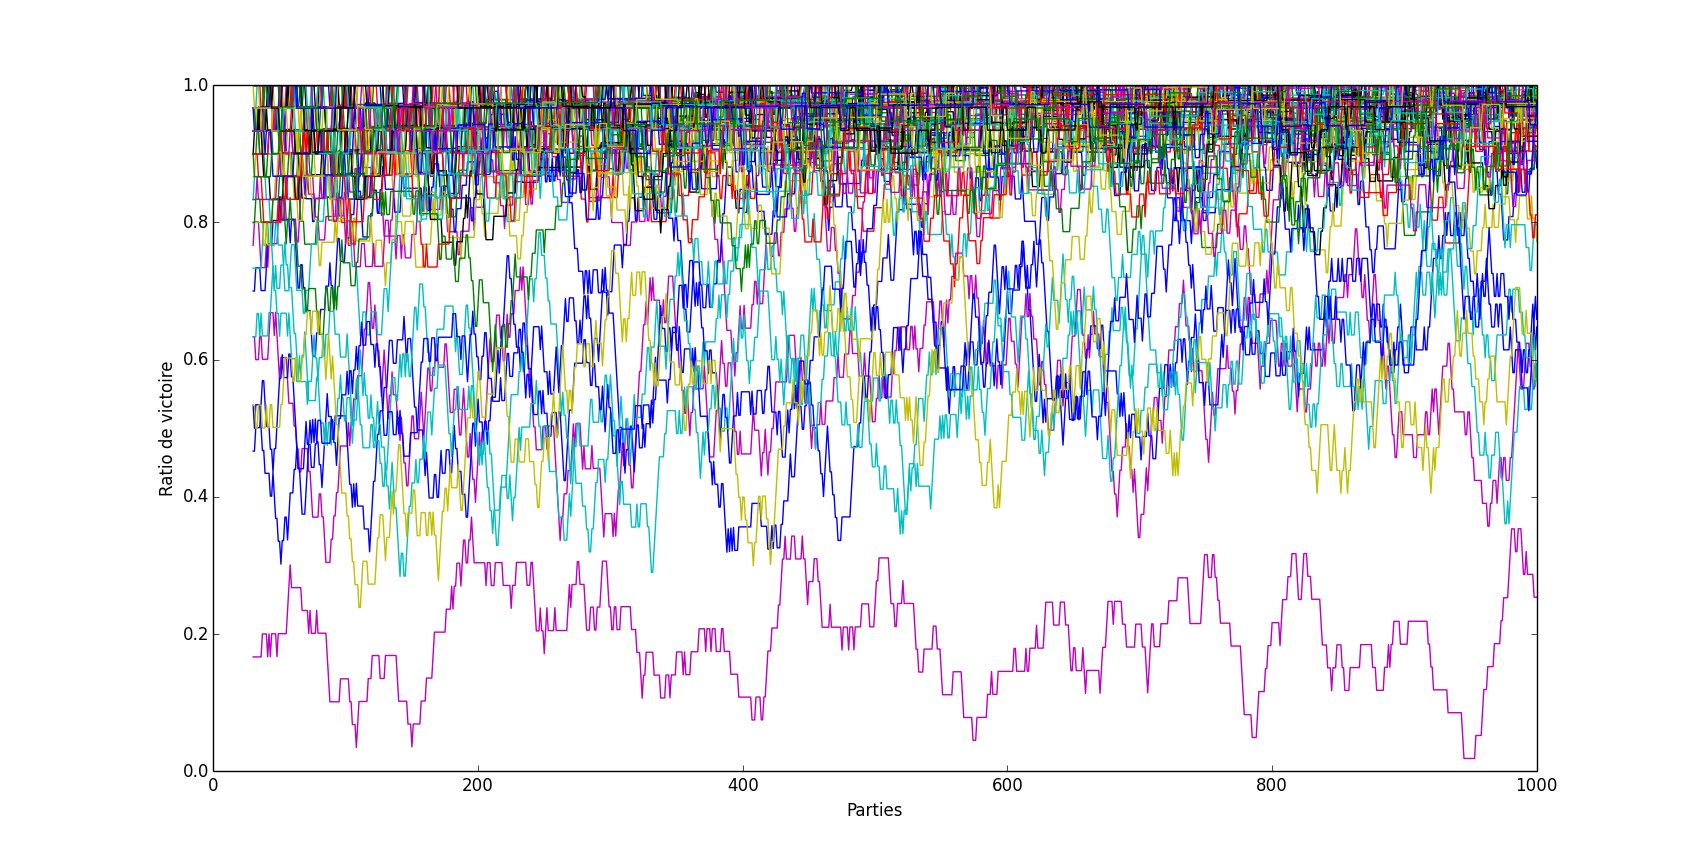
\includegraphics[scale=0.265, trim=0 2cm 0 0]{plot/fake}
  \end{figure}
\end{frame}

\end{document}

% vim: et sw=2 sts=2
